\chapter{Measures of Distributions} \label{ch:measuresdistribution}

Given the probability function or PDF of a random variable, a lot of information can be extracted. Commonly seen measures of a distribution are introduced in this chapter.

\section{Expectation}

In probability and statistics sense, \textit{expectation} (also known as \textit{mean}) describes the average value of a random variable, if the variable is generated many times. For discrete random variable $X$, the expectation is given below.
\begin{eqnarray}
  \textup{E}(X) &=& \sum_{i=1}^{n}x_iP(x_i) \label{eq:expectationdiscrete}
\end{eqnarray}
where $\textup{E}(\cdot)$ is used to denote the expectation, and $n$ the cardinality of the sample space. In the case of countably infinite sample space, replace $n$ with $\infty$ in \eqref{eq:expectationdiscrete}. For continuous random variable, it is
\begin{eqnarray}
  \textup{E}(X) &=& \int_{-\infty}^{\infty}xf(x)dx \label{eq:expectationcontinuous}
\end{eqnarray}
Expectation is sometimes denoted by $\mu$ in literatures.

Some features of expectation calculation are given below.
\begin{eqnarray}
  \textup{E}(cX) &=& c\textup{E}(X) \nonumber \\
  \textup{E}(X+Y) &=& \textup{E}(X) + \textup{E}(Y) \nonumber
\end{eqnarray}
where $c$ is a constant and $X$, $Y$ are two random variables. These features can be easily derived from \eqref{eq:expectationdiscrete} and \eqref{eq:expectationcontinuous}. Furthermore, if $X$, $Y$ are independent, recall $f(x,y) = f_X(x)f_Y(y)$,
\begin{eqnarray}
  \textup{E}(XY) &=& \int_{-\infty}^{\infty}\int_{-\infty}^{\infty} xyf(x, y)dxdy \nonumber \\
  &=& \int_{-\infty}^{\infty}xf_X(x)dx \times \int_{-\infty}^{\infty}yf_Y(y)dy \nonumber \\
  &=& \textup{E}(X)\textup{E}(Y) \nonumber
\end{eqnarray}

\section{Variance and Standard Deviation}

Variance and standard deviation describe how spread samples are from its expectation. It is defined as follows.
\begin{eqnarray}
  \textup{Var}(X) &=& \textup{E}\left(\left(X-\textup{E}(X)\right)^2\right) \label{eq:vardef} \\
  &=& \textup{E}\left(X^2-2X\textup{E}(X)+\textup{E}(X)^2\right) \nonumber \\
  &=& \textup{E}\left(X^2\right)-\textup{E}(X)^2 \label{eq:varderived} \\
  \textup{Std}(X) &=& \sqrt{\textup{Var}(X)} \nonumber
\end{eqnarray}
Variance and standard deviation are sometimes denoted as $\sigma^2$ and $\sigma$ respectively. Notice that \eqref{eq:varderived} also implies that $\textup{E}\left(X^2\right) \geq \textup{E}(X)^2$, a conclusion used in many lemma derivations.

For continuous random variables, from \eqref{eq:varderived} the variance is
\begin{eqnarray}
  \textup{Var}(X) &=& \int_{-\infty}^{\infty} (x-\textup{E}(X))^2f(x)dx \nonumber
\end{eqnarray}
Think of $X$ as an estimation of a parameter $\theta$. If the estimation is non biased, $E(X)=\theta$. Therefore, from the above equation, for a non-biased estimation, the variance of the estimates (left) equals to the MSE of the estimate (right) with sample numbers approaching infinity.

Some features of variance calculation are given below.
\begin{eqnarray}
  \textup{Var}(cX) &=& c^2\textup{Var}(X) \nonumber
\end{eqnarray}
For independent random variables $X$ and $Y$,
\begin{eqnarray}
  \textup{Var}(X\pm Y) &=& \textup{Var}(X) + \textup{Var}(Y) \nonumber
\end{eqnarray}

Mean and standard deviation can be used to standardize a random variable as follows.
\begin{eqnarray}
  X^* &=& \dfrac{X-\mu}{\sigma} \nonumber
\end{eqnarray}
where $\mu$, $\sigma$ are the mean and standard deviation of random variable $X$ respectively. The standardized random variable, $X^*$, has a mean of $0$ and standard deviation of $1$.

\section{Moments} \label{sec:moments}

In mathematics, the $r$-th moment of a continuous function $f(x)$ about $c$ is defined as follows.
\begin{eqnarray}
  \mu_n &=& \int_{-\infty}^{\infty}(x-c)^nf(x)dx \nonumber
\end{eqnarray}

By simply saying \textit{moment} without specifying $c$, it is by default that $c=0$. Let $f(x)$ be a PDF. In this sense, the $0$-th order and the $1$st order moment of a probability density function can be calculated as follows.
\begin{eqnarray}
  && \mu_0 = \int_{-\infty}^{\infty}f(x)dx = 1 \nonumber \\
  && \mu_1 = \int_{-\infty}^{\infty}xf(x)dx = \textup{E}(X) \nonumber
\end{eqnarray}
where it can be seen that the $0$th and $1$st moments of a PDF are 1 and its mean, respectively.

Further more, let $c=\mu_1$ be the mean of the random variable to calculate the $2$nd order \textit{central moment} $\mu_2$ as follows.
\begin{eqnarray}
  \mu_2 = \int_{-\infty}^{\infty}(x-\mu_1)^2f(x)dx = \textup{Var}(X) \nonumber
\end{eqnarray}
which is the variance of the random variable.

Using mean and variance to further define \textit{standardized moments} as shown below. Define $\bar{\mu}_k$ for $k\geq 3$ as follows.
\begin{eqnarray}
  && \bar{\mu}_k = \dfrac{\mu_k}{\sigma^k} \nonumber
\end{eqnarray}
where
\begin{eqnarray}
	&& \mu_k = \textup{E}\left((X-\mu_1)^k\right) = \int_{-\infty}^{\infty}(x-\mu_1)^kf(x)dx \nonumber \\
	&& \sigma^k = \left(\mu_2\right)^{\dfrac{k}{2}} = \left(\int_{-\infty}^{\infty}(x-\mu_1)^2f(x)dx\right)^{\dfrac{k}{2}} \nonumber
\end{eqnarray}
with $\mu_1$ and $\mu_2$ the mean ($1$st order moment) and variance ($2$nd order central moment) of the random variable respectively.

The $3$-rd and $4$-th order standardized moments are known as the \textit{skewness} and \textit{kurtosis} of the PDF respectively. In some literatures, skewness is denoted by $\gamma_1 = \bar{\mu}_3$, and kurtosis $\gamma_2 = \bar{\mu}_4$.

The skewness $\gamma_1$ is a measure of asymmetry of the PDF. When $\gamma_1 > 0$ or positive skew, the distribution has a long tail on the right side of the PDF. When $\gamma_1 <0$ or negative skew, the distribution has a long tail on the left side. When $\gamma_1 = 0$, the PDF might be symmetric (but not necessarily so). Examples are given in Fig. \ref{fig:skewness_demo}.
\begin{figure}
	\centering
	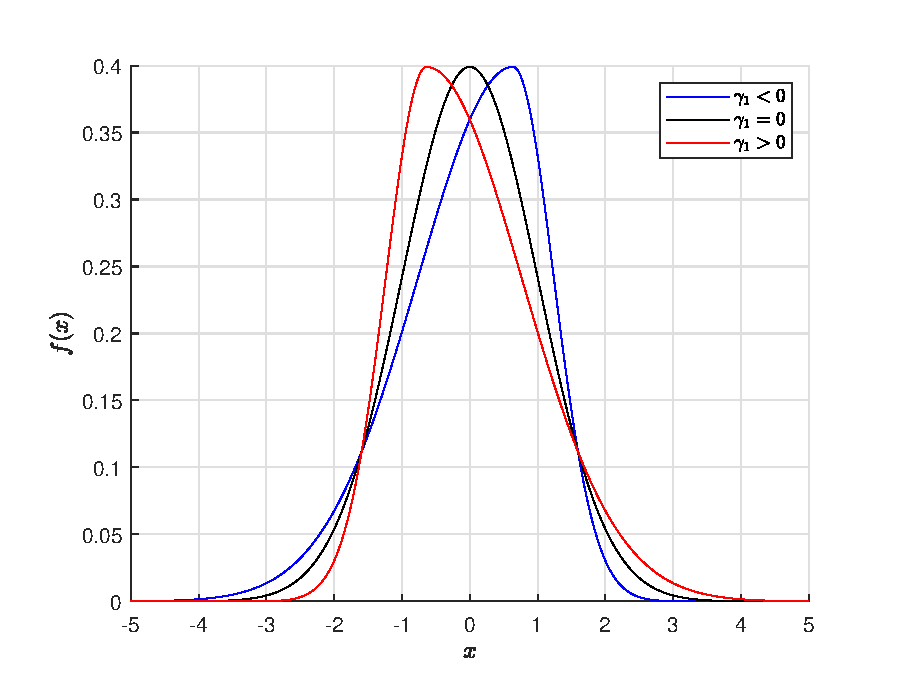
\includegraphics[width=250pt]{chapters/ch-measures-of-distribution/figures/skewness_demo.eps}
	\caption{Demonstration of PDF with different skewness.} \label{fig:skewness_demo}
\end{figure}

The kurtosis $\gamma_2$ measures the ``tailedness'' of a probability distribution, i.e., whether the PDF has heavy tail or thin tail. The normal distribution, which has $\gamma_2=3$, is often used as a benchmark. Excess kurtosis is kurtosis subtracting $3$, making the normal distribution having the excess kurtosis of $0$. A positive excess kurtosis would mean a ``heavier'' tail than the normal distribution. Examples are given in Fig. \ref{fig:kurtosis_demo}.
\begin{figure}
	\centering
	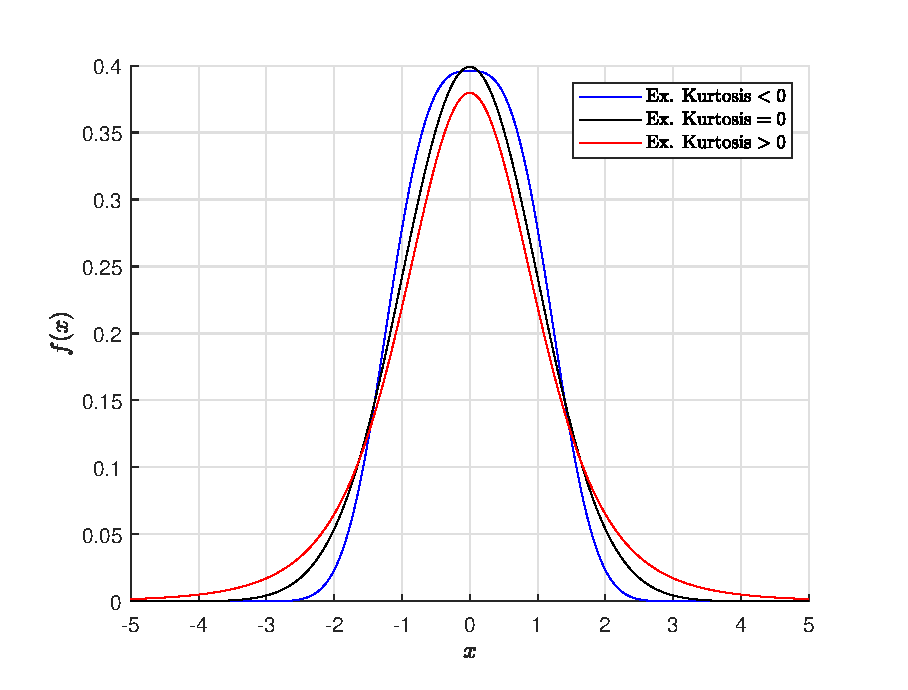
\includegraphics[width=250pt]{chapters/ch-measures-of-distribution/figures/kurtosis_demo.eps}
	\caption{Demonstration of PDF with different excess kurtosis.} \label{fig:kurtosis_demo}
\end{figure}

\section{Covariance and Correlation}

Covariance and correlation are defined for a joint distribution with multiple random variables. For simplicity, consider only two random variables $X$, $Y$ whose joint distribution is given by $f_{XY}(x, y)$. The idea derived from here can be generated to more variables.

\subsection{One Variable}

The PDF of one variable can be derived from the joint distribution using \eqref{eq:jointpdfdowngrade}. It is straight forward to get the expectation and variance for that variable as follows.
\begin{eqnarray}
  \textup{E}(X) &=& \int_{-\infty}^{\infty}\int_{-\infty}^{\infty}xf(x, y)dxdy \nonumber \\
  \textup{Var}(X) &=& \int_{-\infty}^{\infty}\int_{-\infty}^{\infty}\left(x-\textup{E}(X)\right)^2f(x, y)dxdy \nonumber
\end{eqnarray}

\subsection{Covariance}

The \textit{covariance} of two variables is defined and calculated as follows.
\begin{eqnarray}
  \textup{Cov}(X, Y) &=& \textup{E}\left((x - \textup{E}(X))(y - \textup{E}(Y))\right) \label{eq:covariance1} \\
  &=& \int_{-\infty}^{\infty}\int_{-\infty}^{\infty}(x - \textup{E}(X))(y - \textup{E}(Y))f(x, y)dxdy \label{eq:covariance2}
\end{eqnarray}
where $\textup{Cov}(X, Y)$ is sometimes denoted by $\sigma_{XY}$. Notice that unlike variance that is always positive, covariance can be zero or negative. If $X$, $Y$ are independent variables, $f(x,y) = f_X(x)f_Y(y)$. From \eqref{eq:covariance2}
\begin{eqnarray}
   \textup{Cov}(X, Y) &=& \int_{-\infty}^{\infty}(x - \textup{E}(X))f_X(x)dx \times \int_{-\infty}^{\infty}(y - \textup{E}(Y))f_Y(y)dy \nonumber \\
   &=& 0 \nonumber
\end{eqnarray}
If the covariance of the two variables is zero, the two variables are called \textit{uncorrelated}. Independent variables are always uncorrelated. However, uncorrelated variables are not necessarily independent.

Furthermore,
\begin{eqnarray}
  \textup{Cov}(X, Y)^2 &\leq& \textup{Var}(X)\textup{Var}(Y) \nonumber
\end{eqnarray}
The proof is as follows. Notice that lemma \eqref{eq:explemma} is used in the proof.
\begin{mdframed}[frametitle={Lemma}]

For two random variables $X$ and $Y$,
\begin{eqnarray}
	\textup{E}(XY)^2 &\leq&  \textup{E}(X^2)\textup{E}(Y^2) \label{eq:explemma}
\end{eqnarray}
\noindent Proof:
\begin{eqnarray}
	0 &\leq& \textup{E}\left(\left(X-Y\dfrac{\textup{E}(XY)}{\textup{E}(Y^2)}\right)^2\right) \nonumber \\
	&=& \textup{E}\left(X^2-2XY\dfrac{\textup{E}(XY)}{\textup{E}(Y^2)}+\textup{E}(Y^2)\dfrac{\textup{E}(XY)^2}{\textup{E}(Y^2)^2}\right) \nonumber \\
	&=& \textup{E}(X^2) - 2\textup{E}(XY)\dfrac{\textup{E}(XY)}{\textup{E}(Y^2)} + \textup{E}(Y^2)\dfrac{\textup{E}(XY)^2}{\textup{E}(Y^2)^2} \nonumber \\
	&=& \textup{E}(X^2) - 2\dfrac{\textup{E}(XY)^2}{\textup{E}(Y^2)} + \dfrac{\textup{E}(XY)^2}{\textup{E}(Y^2)} \nonumber \\
	&=& \textup{E}(X^2) - \dfrac{\textup{E}(XY)^2}{\textup{E}(Y^2)} \nonumber
\end{eqnarray}
Therefore
\begin{eqnarray}
	\dfrac{\textup{E}(XY)^2}{\textup{E}(Y^2)} &\leq& \textup{E}(X^2) \nonumber \\
	\textup{E}(XY)^2 &\leq&  \textup{E}(X^2)\textup{E}(Y^2) \nonumber
\end{eqnarray}
\end{mdframed}
Using \eqref{eq:explemma} on \eqref{eq:covariance1}, \eqref{eq:vardef} gives
\begin{eqnarray}
	\textup{Cov}(X, Y)^2 &=& \textup{E}\left((x - \textup{E}(X))(y - \textup{E}(Y))\right)^2 \nonumber \\
	&\leq& \textup{E}\left((x - \textup{E}(X))\right)^2\textup{E}\left((y - \textup{E}(Y))\right)^2 \nonumber \\
	&=& \textup{Var}(X)\textup{Var}(Y) \nonumber
\end{eqnarray}
or equivalently
\begin{eqnarray}
	\sigma_{XY}^2 &\leq& \sigma_X^2\sigma_Y^2 \nonumber
\end{eqnarray}
Noticing that while $\sigma_X$, $\sigma_Y$ are always nonnegative, $\sigma_{XY}$ is not,
\begin{eqnarray}
	-\sigma_X\sigma_Y \leq \sigma_{XY} \leq \sigma_X\sigma_Y \label{eq:covlemma}
\end{eqnarray}



\subsection{Correlation}

The \textit{correlation} of two variables is defined and calculated as follows.
\begin{eqnarray}
  \rho &=& \dfrac{\textup{Cov}(X, Y)}{\sqrt{\textup{Var}(X)}\sqrt{\textup{Var}(Y)}} \nonumber \\
   &=& \dfrac{\sigma_{XY}}{\sigma_X\sigma_Y} \nonumber
\end{eqnarray}
From \eqref{eq:covlemma}, apparently $-1\leq \rho \leq 1$. When two variables are uncorrelated or independent, $\rho=0$. If $\rho=1$, it is called \textit{perfect positive correlation}. This happens usually because the two variables are positively linearly depended, for example, $X=2Y$ or $X=Y+1$. If $\rho=-1$, it is called \textit{perfect negative correlation}, and the similar idea applies.

\section{Important Theorems}

There are a few important theorems frequently used in the study of probability and statistics. They are introduced here.

\subsection{Law of Large Numbers}

The \textit{Law of Large Numbers (LLN)} is a theorem that basically says if performing the same experiment a large number of times, the average of the outcomes of the experiments should eventually converge to a certain value which is the empirical expectation of the experiment. The larger number of trails, the closer the average to the empirical expectation.

In mathematical expression, let $X$ be a random variable which represents the outcome of an experiment. Let $X_i$ be a sample of the outcome. According to LLN,
\begin{eqnarray}
  \lim_{n\rightarrow\infty} \sum_{i=1}^{n}\dfrac{X_i}{n} &=& \bar{X} \nonumber
\end{eqnarray}

\subsection{Central Limit Theorem}

\textit{Central Limit Theorem (CLT)} states the following observation. For independent and identically distributed (i.i.d) random variables not necessarily following normal distribution, the empirical mean of the samples taken from these distributions tends towards normal distribution when the number of samples is large.

Let $X$ be a random variable not necessarily following normal distribution, and it has mean and variance of $\mu$ and $\sigma^2<\infty$ respectively. Let $X_i$ be samples of the random variable. The empirical mean of the samples is calculated by
\begin{eqnarray}
	\bar{X}_n &=& \dfrac{1}{n}\sum_{i=1}^{n}X_i \nonumber
\end{eqnarray}
CLT states that $\bar{X}_n$ follows normal distribution when $n$ is large. The mean and variance of the normal distribution are $\mu$ and $\dfrac{\sigma^2}{n}$ respectively, i.e.,
\begin{eqnarray}
	\dfrac{\bar{X}_n-\mu}{\dfrac{\sigma}{\sqrt{n}}} \nonumber
\end{eqnarray}
follows standard normal distribution.